\documentclass[12pt,a4paper,final,oneside,onecolumn,titlepage]{article}
\usepackage{times}
\usepackage{geometry}
\usepackage{fancyhdr}
\usepackage{setspace}
\usepackage{natbib}
\usepackage{float}
\usepackage{multirow}
\usepackage{amssymb}
\usepackage{graphicx}
\usepackage{sectsty}
\usepackage[table,xcdraw]{xcolor}
\usepackage{polski}
\usepackage[utf8]{inputenc}
\usepackage[T1]{fontenc}
\usepackage[pagewise]{lineno}
\newgeometry{tmargin=2.5cm, bmargin=2.5cm, lmargin=2.5cm, rmargin=2.5cm}
\setlength{\parindent}{3in}
\setlength{\parskip}{0pt}
\linenumbers
\doublespacing
\sectionfont{\centering}
\renewcommand{\bibsection}{\section*{\large{\textbf{\textsc{\centering{Literatura}}}}}}

\begin{document}
\pagestyle{fancy}
\fancyhead{}
\fancyfoot{}
\chead{Nasze otoczenie i funkcje poznawcze}
\rhead{\thepage}
\bibliographystyle{apalike}
\begin{titlepage}
  \thispagestyle{empty}
  \rhead{\thepage}
  \begin{center}
  \vspace*{1cm}
  \Large
  \textbf{\textsc{Nasze otoczenie i funkcje poznawcze:\\ Badanie zależności między entropią informacyjną \textit{(H)} w otoczeniu oraz wykonaniem treningu uważności, a selektywną uwagą wzrokową.\\}}
  \vspace{1.5cm}
  \textit{Laura Plichta, Wiktor Warchałowski, Zofia Załęska\\}
  Wydział Nauk o Zdrowiu, Gdański Uniwersytet Medyczny\\
  \vspace{3cm}
  Praca zaliczeniowa z przedmiotu \\ Metodologia Badań Psychologicznych 2 \\ napisana pod kierunkiem dr. Krzysztofa Basińskiego\\
  \vspace{3cm}
  Gdańsk, 20 Stycznia 2023
  \end{center}
\end{titlepage}
\begin{center}
  \vspace*{0.5cm}
  \large{\textbf{\textsc{Abstrakt}}}
\end{center}
\paragraph{}
Celem niniejszego artykułu jest zbadanie problematyki związanej z wpływem środowiska w jakim się znajdujemy na zdolności poznawcze człowieka. Artykuł ten sprawdza czy istnieje wpływ entropii informacji zaindukowanej przez różnorodność obiektów w otoczeniu i wykonaniem treningu uważności jakim jest kolorowanie mandali na selektywną uwagę wzrokową. Badanie zostało przeprowadzone na 30 osobach, które dobrowolnie zgodziły się na wzięcie udziału w eksperymencie. Indukowana entropia otoczenia została opisana jako różnorodność kulek do basenu dziecięcego w pomieszczeniu, zaś trening uważności jako wykonanie kolorowanki z mandalą. Zmienną niezależną była uwaga wzrokowa, zbadana za pomocą testu Eriksena. Średnie porównywanych grup, test t studenta oraz mieszane modele liniowe z nałożonymi kontrastami średnich marginalnych wykazały istnotną statystycznie interakcję porównywanych grup. Współczynnik d Cohena wskazał siłę efektu, którą można uznać za nieistotną w populacji.
\\
\textit{Słowa kluczowe: środowisko, entropia informacji, uwaga wzrokowa, trening uważności}
\newpage
\begin{center}
\section*{\large{\textbf{\textsc{Wstęp}}}}
\end{center}
\paragraph{}
Ze względu na rozwój techniki, kończące się zasoby naturalne, zwiększająca się liczba ludności oraz inne problemy dynamicznie rozwijającego się świata wzrosło zainteresowanie badaniami zależności między człowiekiem, a jego środowiskiem. Dziedziną zajmującą się relacją ludzi i ich zachowań z różnymi modalnościami ich otoczenia oraz jego optymalizacją jest psychologia środowiska \citep{banka_psychologia_2018, gifford_environmental_2011}. Dostrzeganie interakcji człowieka ze środowiskiem może być czymś ważnym w rozwoju architektury i planowania przestrzennego, aby era antropocenu nie była stworzona destruktywnym wpływem człowieka na naturę, ale okresem w którym działamy na wspólną korzyć \citep{zalasiewicz_new_2010}. Oprócz celu zrównoważnonego rozwoju aby odpowiedzieć na zmiany klimatyczne, badacze zajmują się optymalizacją naszego najbliższego otoczenia. Przykładem takiego działania są badania \citet{lohr_interior_1996} pokazujące zależność struktury miejsca pracy z produktywnością. Jednakże analiz tego typu jest relatywnie mało, ale ich ilość wzrasta w XXI wieku \citep{spano_human_2020}. Inspirując się takim typem eksperymentów, celem niniejszego badania było sprawdzenie, jak modyfikacja środowiska pracy wpłynie na efektywność procesów poznawczych człowieka z naciskiem na selektywną uwagę wzrokową. Aby zuniwersalizować manipulację wyglądem otoczenia, zostało zastosowane pojęcie entropii informacji zgodnie z teorią Shannona. Oznacza to, że fizyczna miara nieuporządkowania i chaosu, jest interpretowana jako suma średnich prawdopodobieństw wystąpienia danego typu informacji i zdarzeń. Jest wyrażana wzorem:
\begin{center}
\begin{math}
H_f=-\displaystyle\sum_{i=1}^{n}p_i\log_2({p_i})
\end{math}
\end{center}
Gdzie $n$ oznacza ilość obiektów, $i$ to dany obiekt, zaś $p$ jest prawdopodobieństwem jego wystąpienia. Wynik powyższego działania podawany jest w bitach \citep{stamps_entropy_2004}. Dodatkowo na potrzeby analizy otoczenia entropia informacji jest liczona jako zróżnicowanie elementów architektonicznych lub dekoracyjnych \citep{stamps_entropy_2004, stamps_entropy_2002}. Ze względu na fakt badania odbioru otoczenia pod względem artystyczno-wizualnym, zdecydowano o dołączeniu kolorowania kolorowanki uważności. Jest to jeden z rodzajów treningu \textit{mindfulness} (z ang. uważność), który polega na pełnej koncentracji na przebiegu kolorowania \citep{zejmo_praktyka_2022}. Liczne badania wykazały, że uważność może być stanem przejściowym, wywołanym podczas krótkotrwałej praktyki (stan uważności) albo cechą osobowości obecną w codziennym życiu (uważność jako cecha) \citep{kiken_state_2015}. Mimo tego, że istnieje znaczna ilość badań sugerujących, że uważność poprawia samopoczucie, niewiele wskazuje na to, jak przebiega ten proces \citep{holzel_how_2011}. Jednym z argumentów jest to, że trening uważności zmienia aktywność mózgu \citep{gotink_8-week_2016} oraz przetwarzanie poznawcze \citep{zeidan_mindfulness_2010}. Trening uważności w postaci kolorowania mandali pomaga w uspokojeniu się i poprawia ogólny stan osób kolorujących \citep{carsley_effectiveness_2018, campenni_effects_2020}, którym również po wykonaniu tej czynności łatwiej jest się skupić oraz wykonywać powierzone zadania. Co więcej, mandale, a szczególnie ich środkowe punkty, są wykorzystywane do medytacji w celu zwiększenia poziomu uwagi i skupienia \citep{shankar_effectiveness_2020}. W ostatnich czasach rośnie również ich popularnosć i rośnie ich rola w życiu codziennym wielu ludzi \citep{dresler_doing_2019}. Stąd dodatkowo ten artykuł sprawdza ich użyteczność co również może pomóc w rozwoju świadomości na temat uwagi i uwarunkowań jej działania. Z tego względu postawionym pytaniem badawczym jest czy zwiększona entropia informacji w kolorach elementów otoczenia oraz wykonanie treningu uważności ma wpływ na selektywną uwagą wzrokową? Przewiduje się, że zwiększona entropia informacji w kolorach elementów otoczenia zmniejsza czas wykonania testu selektywnej uwagi wzrokowej. Dzieje się tak ze względu na fakt, że zwiększona entropia wpływa bezpośrednio na zwiększenie przyjemności i pozytywnego pobudzenia \citep{stamps_entropy_2004, stamps_entropy_2002}, które wpływa na możliwości percepcyjne jednostki, dzięki czemu osoby, którym indukowano przyjemność i pozytywne pobudzenie lepiej radziły sobie z wykonaniem testów percepcyjnych, uwagi wzrokowej oraz ogólnie procesów poznawczych \citep{mcconnell_upbeat_2011, gavazzi_pleasure_2021}. Wykonanie testu uważności również zmniejsza czas wykonania testu selektywnej uwagi wzrokowej ze względu na fakt, że czynność kolorowania mandali pomaga w uspokojeniu się oraz poprawia uważność oraz ogólny stan osoby która koloruje (\textit{mindfulness and wellbeing}) \citep{carsley_effectiveness_2018, campenni_effects_2020}. Wysoki poziom uważności (\textit{mindfulness}) zaś podwyższa poziom uwagi wzrokowej i pomaga w skupieniu się \citep{campillo_effects_2018, sumantry_meditation_2021}. Jednakże w przypadku krótkiego zabiegu - wykonania pojedynczej kolorowanki, może nie mieć żadnego wpływu na poziom uwagi wzrokowej badanych \citep{thompson_influence_2021}.
\begin{center}
\section*{\large{\textbf{\textsc{Metoda}}}}
\end{center}
\subsection*{\normalsize{\textbf{Operacjonalizacja}}}
\paragraph{}
Zmienna niezależna, jaką jest indukowana entropia otoczenia, została zoperacjonalizowana poprzez wprowadzenie w pierwszym warunku sprecyzowanej ilości obiektów w tym samym kolorze ($\Delta H_{f1}=0$), zaś w drugim warunku tej samej ilości obiektów, lecz w różnych kolorach ($\Delta H_{f1}<\Delta H_{f2}$). Dzięki użyciu takiej samej ilości obiektów w obu warunkach entropia maksymalna ($\Delta H_{max}$) będzie równa. Manipulacja zachodzi wyłącznie kolorem, ponieważ tylko ich entropia dodatnio koreluje z przyjemnością (pleasure) \citep{stamps_entropy_2004, stamps_entropy_2002}.\\
Druga zmienna niezależna, jaką jest trening uważności, została zoperacjonalizowana poprzez wykonanie jednego wzoru kolorowanki uważności lub kolorowanie pustej kartki przez 5 minut.\\
Zmienną zależną, selektywną uwagę wzrokową, zmierzono za pomocą czasu reakcji podczas wykonywania testu Eriksena (tzw. \textit{flaker test}) oraz stopnia jego poprawności. Został on zaprogramowany w oprogramowaniu PsychoPy \citep{peirce_psychopy2_2019}. Polegał on na jak najszybszym rozpoznaniu kierunku środkowej strzałki w układzie pięciu strzałek. Miał on 6 możliwych wariantów. W dwóch z nich wszystkie stzałki były w jednym kierunku, w kolejnych dwóch przypadkach środkowe strzałki były w innym kierunku niż pozostałe, zaś w ostatnich dwóch środkowe strzałki były na tle bodźca neurtralnego - poziomych kreskach.
\subsection*{\normalsize{\textbf{Osoby badane}}}
\paragraph{}
Uczestnicy zostali dobrani za pomocą doboru kuli śniegowej z populacji, zaś do losowego przypisania ich do grup niezależnych, czyli dwóch grup z różną indukowaną entropią otoczenia, wykorzystano randomizację w blokach. Łącznie było 30 uczestników o średniej wieku 24 lata. Większość (20 osób) stanowiły kobiety.
\subsection*{\normalsize{\textbf{Procedura}}}
\paragraph{}
Każdy z badanych na początku został poinformowany o celu badania, jego przebiegu, dobrowolności i użycia wyników zebranych w badaniu oraz ustnie wyraził świadomą zgodę.
\paragraph{}
Za każdym razem w sali znajdowało się 30 kulek z basenu dla dzieci o różnych kolorach.
\paragraph{}
\textbf{Grupa z niską entropią otoczenia.} Badani zostali zaproszeni pojedynczo do sali w której panował relatywny początek, a 30 kulek rozproszonych w pomieszczeniu było takiego samego koloru. Następnie badany został poproszony o kolorowanie pustej kartki przez 10 minut (warunek “A”). Po tym czasie został przeprowadzony flanker test i zmierzono czas reakcji badanego. Po przeprowadzeniu testu, badany został poproszony o kolorowanie mandali przez 10 minut (warunek “B”). Po tej aktywności badany został ponownie poproszony o wykonanie flanker testu. Taka procedura została przeprowadzona dla każdego z badanych dobranych do grupy z niską entropią jednakże u połowy badanych zmieniono kolejność manipulacji eksperymentalnej tj. najpierw przeprowadzono warunek “B”, a jako drugi warunek “A”. Do obu opcji badani zostali przydzieleni losowo przez randomizację.
\paragraph{}
\textbf{Grupa z wysoką entropią otoczenia.} Badani zostali zaproszeni pojedynczo do sali w której panował relatywny początek, a  30 kulek rozproszonych w pomieszczeniu było trzech różnych kolorów. Następnie procedura została przeprowadzona w ten sam sposób co w grupie z niską entropią otoczenia - badani zostali poproszeni o obydwu warunków eksperymentalnych (“A” i “B”), połowa w kolejności “A”-”B”, zaś druga “B”-”A”.
\subsection*{\normalsize{\textbf{Etyka}}}
\paragraph{}
Zgoda etyczna na przeprowadzenie badania została otrzymana od prowadzącego przedmiot Metodologia Badań Psychologicznych, realizowanym na Gdańskim Uniwersytecie Medycznym. Badanie, ani kwestionariusz demograficzny nie zbiera danych wrażliwych. Uczestnicy zostali poinformowani o celu badania oraz o jego naturze. Zapewniono ich również, iż udział w badaniu jest zupełnie dobrowolny i w każdej chwili mogą z niego zrezygnować, przez cały czas pozostając anonimowym. Pozyskane zostało też potwierdzenie, że wszyscy uczestnicy ukończyli 18 lat i mają prawo do wyrażenia samodzielnej, świadomej zgody na udział w badaniu. 
\subsection*{\normalsize{\textbf{Analiza statystyczna}}}
\paragraph{}
W celu udzielenia odpowiedzi na postawione pytanie badawcze oraz przetestowania postawionej hipotezy przeprowadzono analizy statystyczne przy użyciu języka programowania i środowiska obliczeniowego R Project for Statistical Computing \citep{r_core_team_r_2022}. Pierwszym wykonanym zabiegiem statystycznym było sprawdzenie normalności rozkładu testem Shapiro-Wilka oraz testem Kołmogorowa-Smirnowa, aby być w stanie dobrać odpowiednio następne testy statystyczne. Za poziom istotności przyjęto $\alpha = 0.05$. Wartość \textit{p} obydwu testów wyniosła $p < 2.2*10^{-16}$ co oznacza, że została przyjęta hipoteza zerowa mówiąca o rozkładzie odbiegającym od rozkładu normalnego. Graficznym przedstawieniem rozkładu uzyskanych wyników jest poniższy histogram \textit{(Rysunek 1)}. Jednakże w trakcie wstępnej analizy danych zauważono, że wszyskie wartości czasiu reakcji wynoszące powyżej 1 sekundy są wartościami odstającymi - znajdują się poza $3SD$ oraz $1.5IQR$. Dodatkowo ilość obserwacji jest bardzo duża, a z tego powodu test normalności rozkładu jest niewymierny i niekonieczny do policzenia co wynika z centralnego twierdzenia granicznego \citep{kwak_central_2017}. Rozkład wartości bez wartości odstających przedstawiony jest na \textit{Rysunku 2}. Z tego powodu, w celu statystycznego opisania otrzymanych wyników posłużono się testami parametrycznymi. Dodatkowo przeprowadzono pomiar siły efektu za pomocą współczynnika d Cohena. Mówi on o "stopniu do jakiego badane zjawisko istnieje" \citep[s. 5]{cohen_statistical_1977}. 
\begin{figure}[H]
\centering
\caption{Histogram przedstawiający rozkład wyników z wartościami odstającymi}
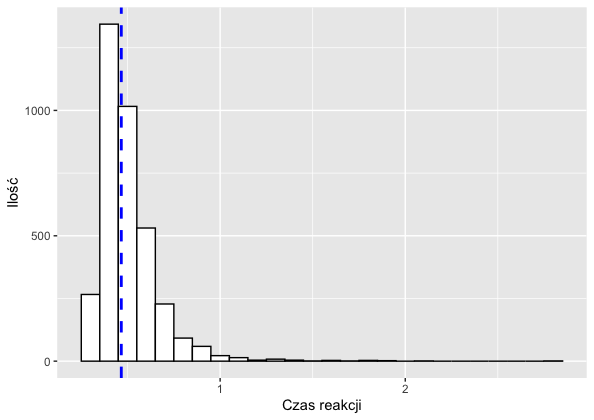
\includegraphics[scale=0.5]{hist1}
\label{Rysunek}
\end{figure}
\begin{figure}[H]
\centering
\caption{Histogram przedstawiający rozkład wyników bez wartości odstających}
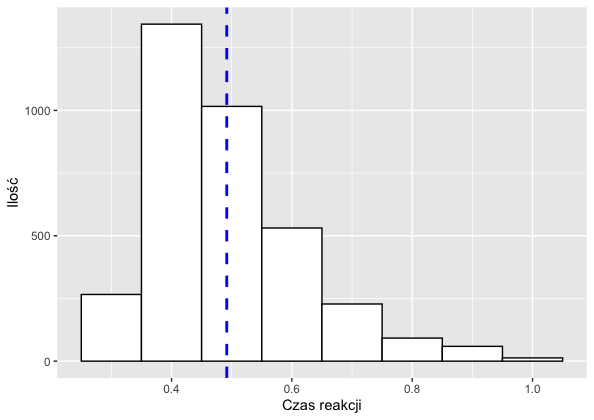
\includegraphics[scale=0.5]{hist2}
\label{Rysunek}
\end{figure}
\begin{center}
\section*{\large{\textbf{\textsc{Wyniki}}}}
\end{center}
\paragraph{}
Po sprawdzeniu normalności rozkładu i wybraniu typu testów statystycznych, zostały policzone podstawowe statystyki opisowe dla zbioru danych nieodbiegających od rozkładu normalnego - miary tendencji centralnej, zmienności oraz asymetrii. Były to średnia, odchylenie standardowe, klasyczny współczynnik zmienności oraz klasyczny współczynnik asymetrii. Dla całego zbioru danych średnia ($M$) wyniosła $0.49$, odchylenie standardowe ($SD$) wyniosło $0.13$, współczynnik zmienności ($V_x$) miał wartość $25.57$, zaś asymetria ($A_{S_{x}}$) wyniosła $1.16$. Wyniki powyższych cech statystycznych dla 4 badanych grup zostały przedstawione w \textit{Tabeli 1}. Dodatkowo narysowano wykres \textit{box and whiskers plot} dla powyższych grup \textit{(Rysunek 3)}.
\begin{table}[H]
\caption{Statystyki opisowe}
\centering
\begin{tabular}{l c c c c}
\hline\hline
Grupa & $M$ & $SD$ & $V_x$ & $A_{S_{x}}$ \\ [0.5ex]
\hline
Mandala i wysoka entropia&0.50&0.13&26.68&1.18 \\
Mandala i niska entropia&0.50&0.13&25.46&0.94 \\
Kartka i wysoka entropia&0.48&0.11&23.25&1.30 \\
Kartka i niska entropia&0.49&0.13&26.32&1.16 \\ [1ex]
\hline
\end{tabular}
\label{Tabela}
\end{table}
\begin{figure}[H]
\centering
\caption{Box and whiskers plot przedstawiający rozkład wyników w grupach}
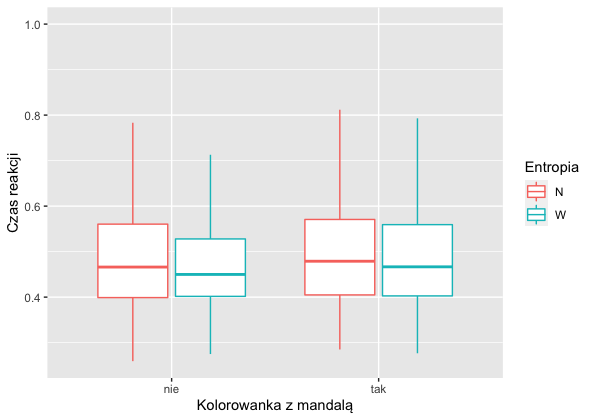
\includegraphics[scale=0.5]{box1}
\label{Rysunek}
\end{figure}
\paragraph{}
Poza opisem podstawowymi statystykami opisowymi przeprowadzono testy statystyczne badające związek pomiędzy badanymi zmiennymi. Był to test t studenta w warunku grup zależnych i grup niezależnych. Były to testy badające osobne zależności między badanymi zmiennymi. Dodatkowo przeprowadzono analizę wariancji dla wszystkich badanych zmiennych i ich interakcji za pomocą mieszanego modelu liniowego \textit{(linear mixed model)} oraz zbadano kontrasty za pomocą średnich estymowanych \textit{(estimated marginal means)}. Wartości $p$ dla testu t studenta oraz modelu liniowego zostały przedstawione w \textit{Tabeli 2}, zaś wyniki kontrastów modelu liniowego zostały przedstawione w \textit{Tabeli 3}.
\begin{table}[H]
\caption{Wartości $p$ obliczonych testów statystycznych}
\centering
\begin{tabular}{l c c c}
\hline\hline
 & Entropia & Kolorowanka & Interakcja \\ [0.5ex]
\hline
\multirow{4}{*}{Czas reakcji}& \multicolumn{3}{c}{Test t studenta} \\
 &$0.014^*$&0.22&- \\ [3ex]
 & \multicolumn{3}{c}{Mieszany model liniowy}\\
 &$0.52$&$8.55*10^{-5*}$&$0.037^*$ \\
\hline
\multicolumn{4}{l}{\footnotesize{$^{*} - p<0.05$}}
\end{tabular}
\label{Tabela}
\end{table}
\begin{table}[H]
\caption{Wartości $p$ kontrastów nałożonych na model liniowy}
\centering
\begin{tabular}{c c c}
\hline\hline
\multicolumn{2}{c}{Kontrast (Entropia, Mandala)} & Wartość $p$ \\ [0.5ex]
\hline
N nie & W nie & $0.77$ \\
N nie & N tak & $0.56$ \\
N nie & W tak & $.00$ \\
W nie & N tak & $0.60$ \\
W nie & W tak & $1.00*10^{-4*}$ \\
N tak & W tak & $0.99$ \\
\hline
\multicolumn{3}{l}{\footnotesize{$^{*} - p<0.05$}}
\end{tabular}
\label{Tabela}
\end{table}
\paragraph{}
Powyższe wyniki pokazują, że test t studenta wykazał istotność statystyczną dla zależności entropii i czasu reackji oraz model liniowy wykazał istotność statystyczną zależności kolorowania mandali z czasem reakcji ze względu na zachodzącą istotnie statystyczną interakcję. Kontrasty wykazały, że kolorowanie mandali istotnie zwiększa czas reakcji tylko w warunku wysokiej entropii.
\paragraph{}
Wartości siły efektu dla obu grup są nieistotne. Dla wpływu kolorowania na czas reakcji w teście uwagi wartość współczynnika d Cohena wyniosła $0.037$, zaś dla wpływu entropii otoczenia na czas reakcji w teście uwagi wzrokowej wartość współczynnika d Cohena wyniosła $0.082$.
\paragraph{}
Dodatkowo pomimo braku tej predykcji w pytaniu badawczym oraz w hipotezie, zauważono iż może istnieć związek pomiędzy typem bodźca wzrokowego, a czasem reakcji oraz, że w przypadku faktu wykonania bądź niewykonania treningu uważności wyniki w teście uwagi się różnią. W tym celu przeprowadzono test ANOVA oraz ponownie mieszany model liniowy \textit{(linear mixed model)} ze zbadaniem kontrastów ze średnich estymowanych z modelu \textit{(estimated marginal means)}. Wynika z nich, że istnieje istotnie statystyczny związek między typem bodźca, a czasem reakcji - wartość $p$ jednoczynnikowego testu ANOVA wyniosła $p<2*10{-16}$. Model liniowy z nałóżonymi kontrastami, zaś wykazał istotną interakcję między typem bodźca, a faktem kolorowania mandali ($p<0.05$). Graficzne różnice zostały przedstawione na poniższym wykresie \textit{box and whiskers plot} na \textit{Rysunku 4}. Wyniki dopasowania modelu liniowego oraz nałożonych kontrastów załączone zostały w \textit{Załączniku 1}.
\begin{figure}[H]
\centering
\caption{Box and whiskers plot przedstawiający mediany wyników w grupach}
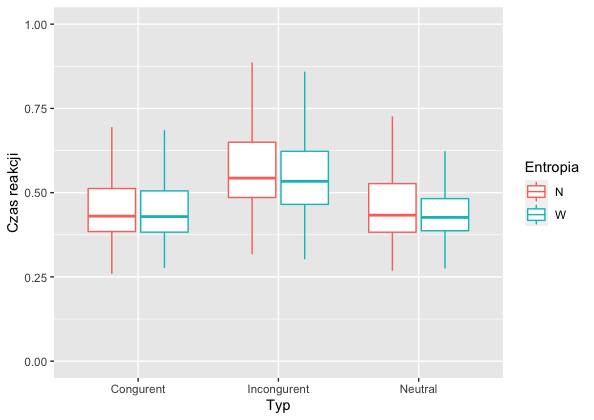
\includegraphics[scale=0.5]{box2}
\label{Rysunek}
\end{figure}
\begin{center}
\section*{\large{\textbf{\textsc{Dyskusja}}}}
\end{center}
\paragraph{}
Badanie miało na celu sprawdzenie wpływu entropii informacji zaindukowanej przez różnorodność obiektów w otoczeniu i wykonaniem treningu uważności na selektywną uwagę wzrokową. Postawiono hipotezę o pozytywnym wpływie wysokiej entropii otoczenia oraz wykonaniem treningu uważności na selektywną uwagę wzrokową
\newpage
\bibliography{Biblio}
\end{document}